%!TEX root = ../masters.tex

\chapter{Introdução}
\label{cha:introduction}


\begin{figure}
    \centering
    \caption{Processo de Extração de Metadados}
    \label{fig:introduction}
    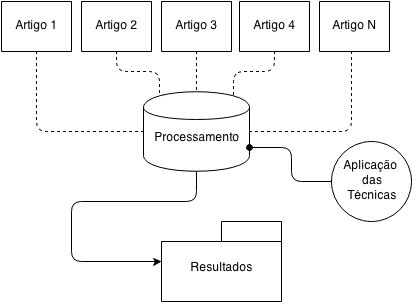
\includegraphics[width=0.9\linewidth]{./assets/images/introduction}
    \center\footnotesize{Fonte: O próprio autor}
\end{figure}

% \section{Contexto}
% \label{sec:context}


Em virtude da grande produção científica existente nos dias atuais, ferramentas automatizadas de extração de metadados de artigos científicos são cada vez mais úteis. Elas contribuem para uma melhor organização dos artigos científicos e facilitam buscas mais rápidos e eficientes.

A pesquisa aqui realizada situa-se no campo da extração de metadados segundo a abordagem \textit{machine learning}. O trabalho considera as ferramentas mais populares atualmente. Diversas ferramentas e técnicas para extração de metadados em artigos podem ser encontradas na literatura científica da área. 

Algumas ferramentas são propriedades de universidades ou instituições privadas, o que dificulta a análise. Outras não permitem que testes automatizados sejam feitos, visto que não há acesso ao código fonte ou não podem ser utilizadas via linha de comando.

De modo geral, as ferramentas de extração são focadas em leiautes pré-definidos, geralmente seguindo modelos (ou \textit{templates}) de revistas e encontros científicos, que possuem um padrão visual já estabelecido. Esse é o caso do IEEE (\textit{Institute of Electrical and Electronics Engineers}), por exemplo, que serve de referência para diversos outros eventos da área da Ciência da Computação.

Porém, existem diversos outros eventos e revistas que empregam \textit{templates} específicos. A extração nesses artigos exige adaptações das ferramentas para que o processo seja satisfatório. 

Algumas ferramentas são aparentemente muito eficazes para um certo grupo de artigos, já seguindo um padrão visual pré-determinado. Porém, para alguns \textit{templates} pouco comuns, de áreas de conhecimento diversas, elas não são tão eficazes. A eficácia varia de acordo com a tecnologia utilizada e, principalmente, de acordo com o princípio teórico utilizado.

Como definido por \cite{foundations-machine-learning}, \textit{machine learning} permite uma forma de aprendizado com base em experiências passadas, através da utilização de dados coletados, que são analisados posteriormente seguindo padrões definidos.

A área é muito ampla e sua aplicabilidade é diversificada, podendo ser usada na classificação, processamento de linguagem natural, reconhecimento de fala, detecção de fraudes, diagnósticos médicos e sistemas de recomendações, além de mecanismos de buscas e extração de informação. Essa última é a aplicação foco neste trabalho.

Claro que as técnicas de extração existentes hoje são, de maneira geral, insuficientes para tratar todos os leiautes de artigos existentes, limitando-se a apenas uma parcela destes, que usam padrões visuais comuns. Espera-se que certos artigos científicos não tenham seus metadados extraídos com total exatidão.

Com base na diferenciação dos leiautes de artigos científicos, o objetivo da pesquisa é comparar o desempenho de ferramentas na tarefa de extração de metadados. Isso será feito com um conjunto de documentos pré-selecionados para testes, dos mais diversos padrões e de diversas áreas do conhecimento.

Espera-se com isso poder identificar o desempenho de tais ferramentas, suas limitações e melhores aplicações: quais ferramentas apresentam melhores resultados para cada padrão visual? Que ferramenta é melhor aplicada para determinado tipo distinto de metadado?

O documento é estruturado iniciando com essa breve introdução e motivação sobre o tema.

O segundo capítulo traz o referencial teórico, onde são apresentados alguns conceitos básicos, além das técnicas mais utilizadas e as ferramentas mais comuns encontradas atualmente.

O terceiro capítulo apresenta a metodologia usada no trabalho, citando as ferramentas que serão testadas e principalmente o método usado nesta pesquisa para a realização dos testes. 

Posteriormente, no capítulo quarto, faz-se a análise e apresentação dos resultados, explicando como os testes foram realizados, os ambientes de teste criados e os resultados coletados.

No quinto capítulo temos a discussão final e a exposição de algumas conclusões mais relevantes, além dos trabalhos futuros e considerações finais sobre o trabalho apresentado.


%\section{Limitações do Trabalho}
%
%Este trabalho limita-se aos artigos científicos difundidos na comunidade científica em formato PDF, excluindo aqueles em que seu conteúdo é disponibilizados através de imagens escaneadas de documentos físicos, o que impede, em um primeiro momento, de ter os textos analisados em sua forma original, sem necessidade de processamento extra a fim de obter todo o material textual contido em tais imagens. Além disso o trabalho pressupõe que a língua inglesa seja utilizada como padrão
%
%% Sobre os servidores com Windows
%
%Já na questão de testes de cada técnica de extração de metadados, as técnicas que serão selecionadas deverão ser de código livre/aberto, ou seja, ter seu uso liberado sem a necessidade de pagamento de licenças. Deste modo excluímos todas as técnicas que necessitam de \textit{softwares} proprietários para funcionar, por exigir licenças e fugirem das previsões de teste deste projeto. Assim, os projetos deverão necessariamente utilizar de linguagens de programação livres (ou de código aberto) e que rodem em sistemas operacionais derivados do Unix, como o Linux, por exemplo.


